\scanpage{102}
% archive sheet number: 101
% printed form: blank music staves; no printed verbal text
% source line 01
\[
\deleted{\unsure{w}}\qquad\deleted{w=a+\frac{2\alpha}{\alpha'}b=a\unsure{-|+}2\alpha^2b=a-2(1-\alpha)b}
\]
% source lines 02-03
Remplaçons $\unsure{v|\nu}$ par sa valeur \unsure{ds|dans la} formule précédente, on trouve
% source line 04
\[
w=\alpha'(\alpha'w-(\alpha'-1)a))-(\alpha'-1)a
\]
% source lines 05-08
\[
\begin{aligned}
(\underbrace{1-\alpha^{\prime 2}}_{\alpha'})w
&=\underbrace{(\alpha'-1)(\underbrace{-\alpha'-1}_{\alpha})}_{\substack{\deleted{\unsure{a-a}}\\\alpha\alpha'-\alpha=-1-\alpha=\alpha'}}a
\qquad\text{i.e.}\quad\alpha'w=\alpha'a\\
&\hspace{7em}\text{i.e.}\quad\underline{w=a}\\
&\text{puis}\quad v=(\alpha'-(\alpha'-1))a=a\\
&\text{donc}\quad\boxed{v=w=a}
\end{aligned}
\]
% source lines 09-11
\[
\begin{aligned}
f(x,y,z)={}&\deleted{\unsure{ax[x+y+x(|ax[x+y+x}}\\
&ax(x+y+z-1)+b\bigl[\underbrace{y(y-\alpha z-1)+z(z-1)}_{(y^2+z^2-y-z-\alpha yz)}\bigr]
\end{aligned}
\]
% source line 12; arcs associate squared and linear terms
\figure{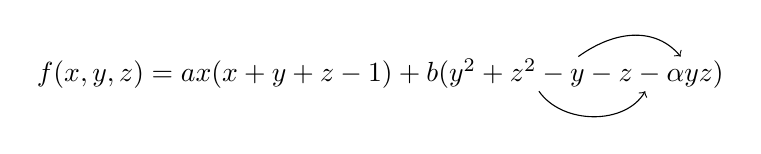
\begin{tikzpicture}
\node[anchor=west] at (0,0) {$f(x,y,z)=ax(x+y+z-1)+b(y^2+z^2-y-z-\alpha yz)$};
\draw[->] (7.0,.22) .. controls (7.5,.58) and (8.0,.58) .. (8.3,.22);
\draw[->] (6.5,-.22) .. controls (6.8,-.65) and (7.6,-.65) .. (7.85,-.22);
\end{tikzpicture}}
% source lines 13-16
\[
\begin{aligned}
f(\unsure{a|\underline a|\widehat a}s_2)=0\quad\text{i.e.}\quad
&a\alpha'(-\alpha')+b\Bigl(\underbrace{\deleted{\unsure{\alpha^{\prime 2}+\alpha'}}\inserted{\unsure{\alpha'(\alpha'+1)|\alpha'(\alpha+1)}}}_{1}+(1-\alpha')(-\alpha')\\
&\hspace{6em}-\underbrace{\alpha(-\alpha')}_{1}(1-\alpha')\Bigr]=0\\
&\underbrace{\hphantom{\alpha^{\prime 2}+\alpha'+(1-\alpha')(-\alpha')-\alpha(-\alpha')(1-\alpha')}}_{\deleted{\alpha'}-\deleted{\alpha'}+\alpha^{\prime 2}}\quad\deleted{\unsure{=0}}\\
&-(\alpha^{\prime 2})a+\alpha^{\prime 2}b=0\qquad\boxed{b=a}
\end{aligned}
\]
% source line 17
\[
f(x,y,z)=aq(x,y,z)
\]
% source lines 18-19
Il reste à vérifier $q(as_0)=q(as_1)=q(as_2)=\unsure{0}$.

Mais c'est OK car $q$ \unsure{invariante}\ldots
